% ---------------------------------------------------------------
% ---------------------------------------------------------------
% This template was developed for the working paper series of 
% the Interdisciplinary Laboratory of Computational Social Science (iLCSS)
% at the University of Maryland, College Park

% The template was built based on  the PNAS Latex model. 

% Adjustments were made by Tiago Ventura, Ph.D. Student in Political Science at UMD, 
% and researcher at the iLCSS.

\documentclass[9pt,twocolumn,twoside]{ilcss}
\usepackage{comment}



\templatetype{ilcssworkingpaper} % Choose template 

\title{Bitcoin Econometrics}	

% Use letters for affiliations, numbers to show equal authorship (if applicable) and to indicate the corresponding author
\author[a]{Gavin Trebilcock}
\author[b]{Tianjiao Li} 
\author[c]{Minghan Shi}

\affil[a]{gt322, Computer Science}
\affil[b]{tl787, Mechanical Engineering}
\affil[c]{ms3536, Electrical and Computer Engineering}

% Please give the surname of the lead author for the running footer
\leadauthor{Gavin} 

% Please include corresponding author, author contribution and author declaration information
\begin{comment}
\authorcontributions{Please provide details of author contributions here.}
\authordeclaration{Please declare any conflict of interest here.}
\end{comment}

\begin{comment}
\equalauthors{\textsuperscript{1}The authors contributed equally to this work.}
\end{comment}

\begin{comment}
\correspondingauthor{\textsuperscript{2}To whom correspondence should be addressed. E-mail: author.two\@email.com}
\end{comment}

\begin{comment}
% Keywords are not mandatory, but authors are strongly encouraged to provide them. If provided, please include two to five keywords, separated by the pipe symbol, e.g:
\keywords{Keyword 1 $|$ Keyword 2 $|$ Keyword 3 $|$ ...}
\end{comment}

\begin{abstract}
In the world of cryptocurrencies, fortunes tend to move up and down quickly. Among them, bitcoin is the original cryptocurrency and it remains the go-to leader of the market. Nevertheless, it is extremly hard to predict the price of bitcoin through standard economic theories, because on bitcoin markets, absent are several features of currency supply and demand, which usually form the basis of currency price. In this report, we present the current progresses in our study of bitcoin market price under the effects of several potential factors. We first show the data retrieval procedures as well as the data visualization, and then present our preliminary data analysis.
\end{abstract}

% \dates{This manuscript was compiled on \today}

% You can change the link on the footer here

\doi{\url{https://github.com/gtrebilcock/BitcoinEconometrics/}}

\begin{document}

\maketitle
\thispagestyle{firststyle}
\ifthenelse{\boolean{shortarticle}}{\ifthenelse{\boolean{singlecolumn}}{\abscontentformatted}{\abscontent}}{}

% If your first paragraph (i.e. with the \dropcap) contains a list environment (quote, quotation, theorem, definition, enumerate, itemize...), the line after the list may have some extra indentation. If this is the case, add \parshape=0 to the end of the list environment.

\dropcap{C}ryptocurrencies have posed great challenges and opportunities for  policymakers, economists, entrepreneurs and consumers since its introduction by Nakamoto \cite{Dyhrberg2016}. The most prominent among them is bitcoin, both in terms of an impressive price development and market capitalisation. However, the price formation of bitcoin cannot be explained by standard economic theories, such as future cash-flows model, purchasing power parity, or uncovered interest rate parity, because several features of currency supply and demand, which usually form the basis of currency price, are absent on bitcoin markets \cite{Ciaian2016}.

We are interested in researching whether or not we can predict the price movement of bitcoin using other public available data. More specifically we are interested testing whether certain metrics which theoretically should be correlated with bitcoin price have any predictive power to determine the prediction of bitcoin prices in the future. 

To do this, we first select candidate factors which potentially have impact on the bitcoin pricing, such as 1. US equity market, 2. GPU pricing, 3. U.S inflation rate 4. U.S interest rates, 5. Gold prices. Then we retrieve the corresponding data set from the Internet and visualize the data to obtain an intuitive observation of them. Next, we do feature engineering and do exploratory data analysis of the features to obtain an intuition of the statistical properties of the data. Finally, we truncate the data into training data $\mathcal{D}_{train}$ and testing data $\mathcal{D}_{test}$, fit a simple linear model to the data, and analyze the learning results. We close this report with a discussion section, including remarks on the current results and issues, and our future plan of this project.

\section*{Important Statement}
\textbf{The authors are well aware that the prediction of bitcoin has been an prominent area of study yet there has been no super effective model for such prediction. In this sense, the reported prediction method may not, or won't perform as well as expected. However, the purpose of this study mainly lies in practicing and utilizing the basics of learning theories in a real-world problem. In the meantime, the authors anticipate understanding the underlying difficulties of predicting the bitcoin price from a practical perspective.}

\section{Selection of Explanatory Variables}
We use the overall US equity market as a predictor for future bitcoin prices as the US equity market generalizes the overall health of the economy, consumer confidence and other socio-political factors that will influence bitcoin pricing. We selected the S\&P as the approximation for the overall US equity market as it is a market capitalization weighted fund, which is believed to give a good approximation for the overall health of the market rather than older indexes such as the Dow Jones Industrial Average which is price weighted.  

GPU pricing is another indicator for the prediction of bitcoin pricing in our hypothesis as GPU’s are the primary input cost in mining bitcoins. It is prohibitively difficult to find a data set that tracks GPU component pricing, as there are many different models from different companies available. Instead, we elect to approximate this factor using the stock price of the world’s largest producer of GPU’s, Nvidia.

We also consider the US inflation rate as a candidate for the indicator. One of the most valuable characteristics of bitcoin is the finite supply which cannot be manipulated by governmental bodies. Therefore we expect to find a correlation between inflation rates and bitcoin prices as some investors use finite supply assets to hedge risk from inflation.

Interest rates is also considered as a potential factor influencing the bitcoin pricing, as currencies are priced against one another based on the interest rate in that country and the financial standing of that country. Accordingly, since we are measuring bitcoin per USD, it is reasonable to add the variable of US interest rates into our model. We chose the 3-month LIBOR as our metric to track daily interest rate changes.

Finally, we expect to the spot price of gold to be an important indicator in predicting bitcoin prices. The selection of this asset has many dimensions which are equivalent to bitcoin, including most notably its finite supply. Historically, gold was used as a currency and is still being used as a store of wealth. Bitcoin shares similar characteristics as it is currently being used as a store of wealth and is attempting to make its way into the arena of currencies on a global level.

\section{Retrieval of Data}
We retrieved daily bitcoin pricing (Figure 1 (a)) from \url{https://coinmarketcap.com/currencies/bitcoin/historical-data/} which is a database that tracks many cryptocurrencies. The site offers the longest history on Bitcoin pricing that we were able to find dating back to April 28, 2013.

Our S\&P500 (Figure 1 (b)) and Nvidia daily price data (Figure 1 (c)) were extracted from Yahoo finance and are measured in USD. Yahoo finance offers adjusted close prices which adjust daily close prices for dividends and stock splits. This makes the calculation for daily returns much simpler. We note that daily data for these two assets are tracked on trading days, which specifically exclude weekends and holidays. This forced us to use 253 data points per year rather than the expected 365. We pulled data only for the dates that aligned with these two assets, as there would be less sparse data to deal with. 

Our daily spot gold pricing (Figure 1 (d)) was taken from \url{https://perthmint.com/} which provides daily spot pricing for gold priced in United States Dollars per ounce. 

\begin{figure*}
\centering
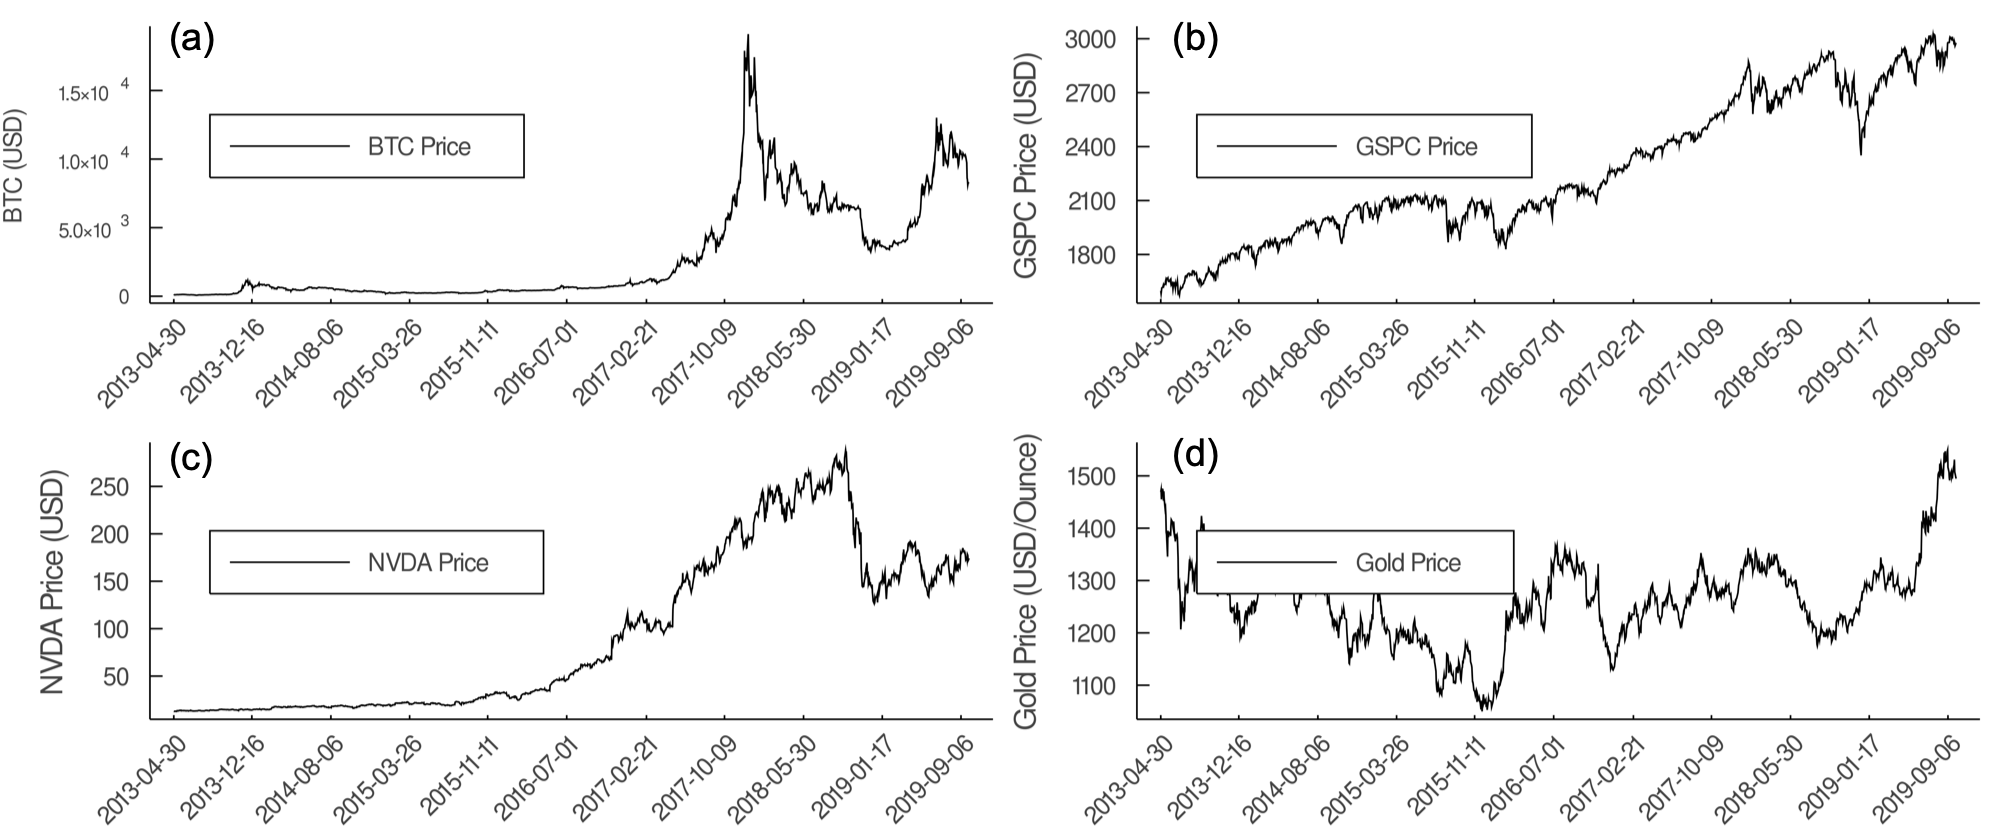
\includegraphics[width=0.9\linewidth]{fig1to4.png}
\caption{(a)The Bitcoin price since April 28, 2013, on a daily basis (retrieved from \url{https://coinmarketcap.com/currencies/bitcoin/historical-data/}) (b)S\&P500 daily price since April 28, 2013, on a daily basis (retrieved from Yahoo finance) (c)Nvidia daily price since April 28, 2013, on a daily basis (retrieved from Yahoo finance) (d)Daily spot gold pricing taken from \url{https://perthmint.com/}.}
\label{fig:1}
\end{figure*}

We found daily inflation rates from the Federal Reserve Economic Data (FRED) database \url{https://fred.stlouisfed.org/}. This variable is measured daily and the units on each data point is in percentage terms. We also retrieved daily 3-month LIBOR rates from the FRED database. This variable is measured daily and the units on each data point is in percentage terms. 

\begin{figure}[tbhp]
\centering
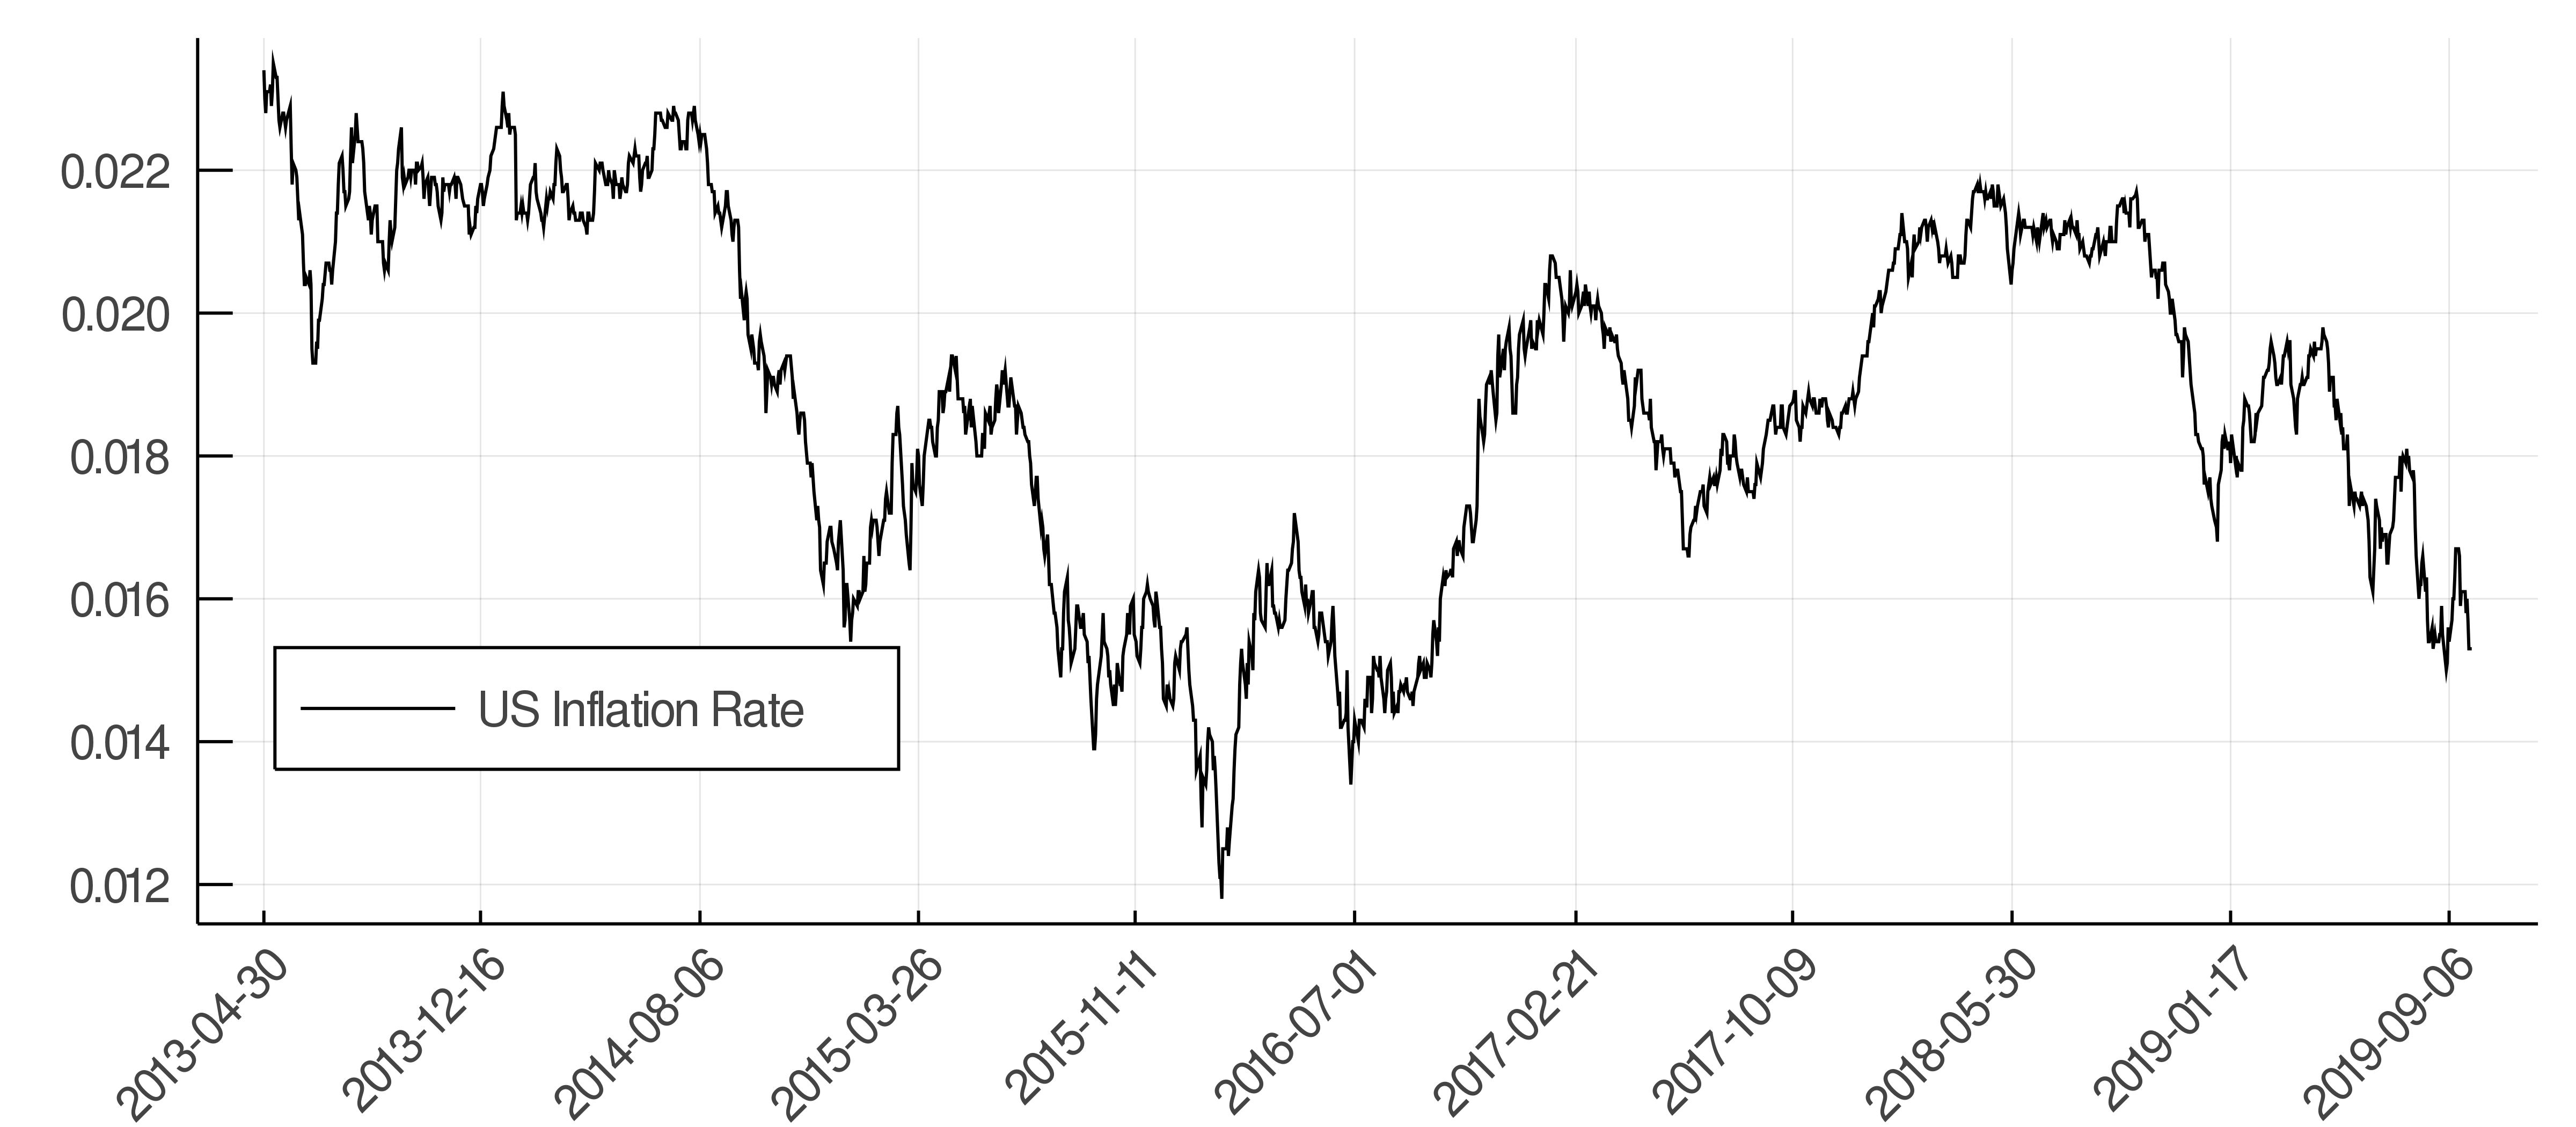
\includegraphics[width=.9\linewidth]{US_inflation_rate.png}
\caption{daily inflation rates from the Federal Reserve Economic Data (FRED) database \url{https://fred.stlouisfed.org/}}
\label{fig:2}
\end{figure}

\begin{figure}[tbhp]
\centering
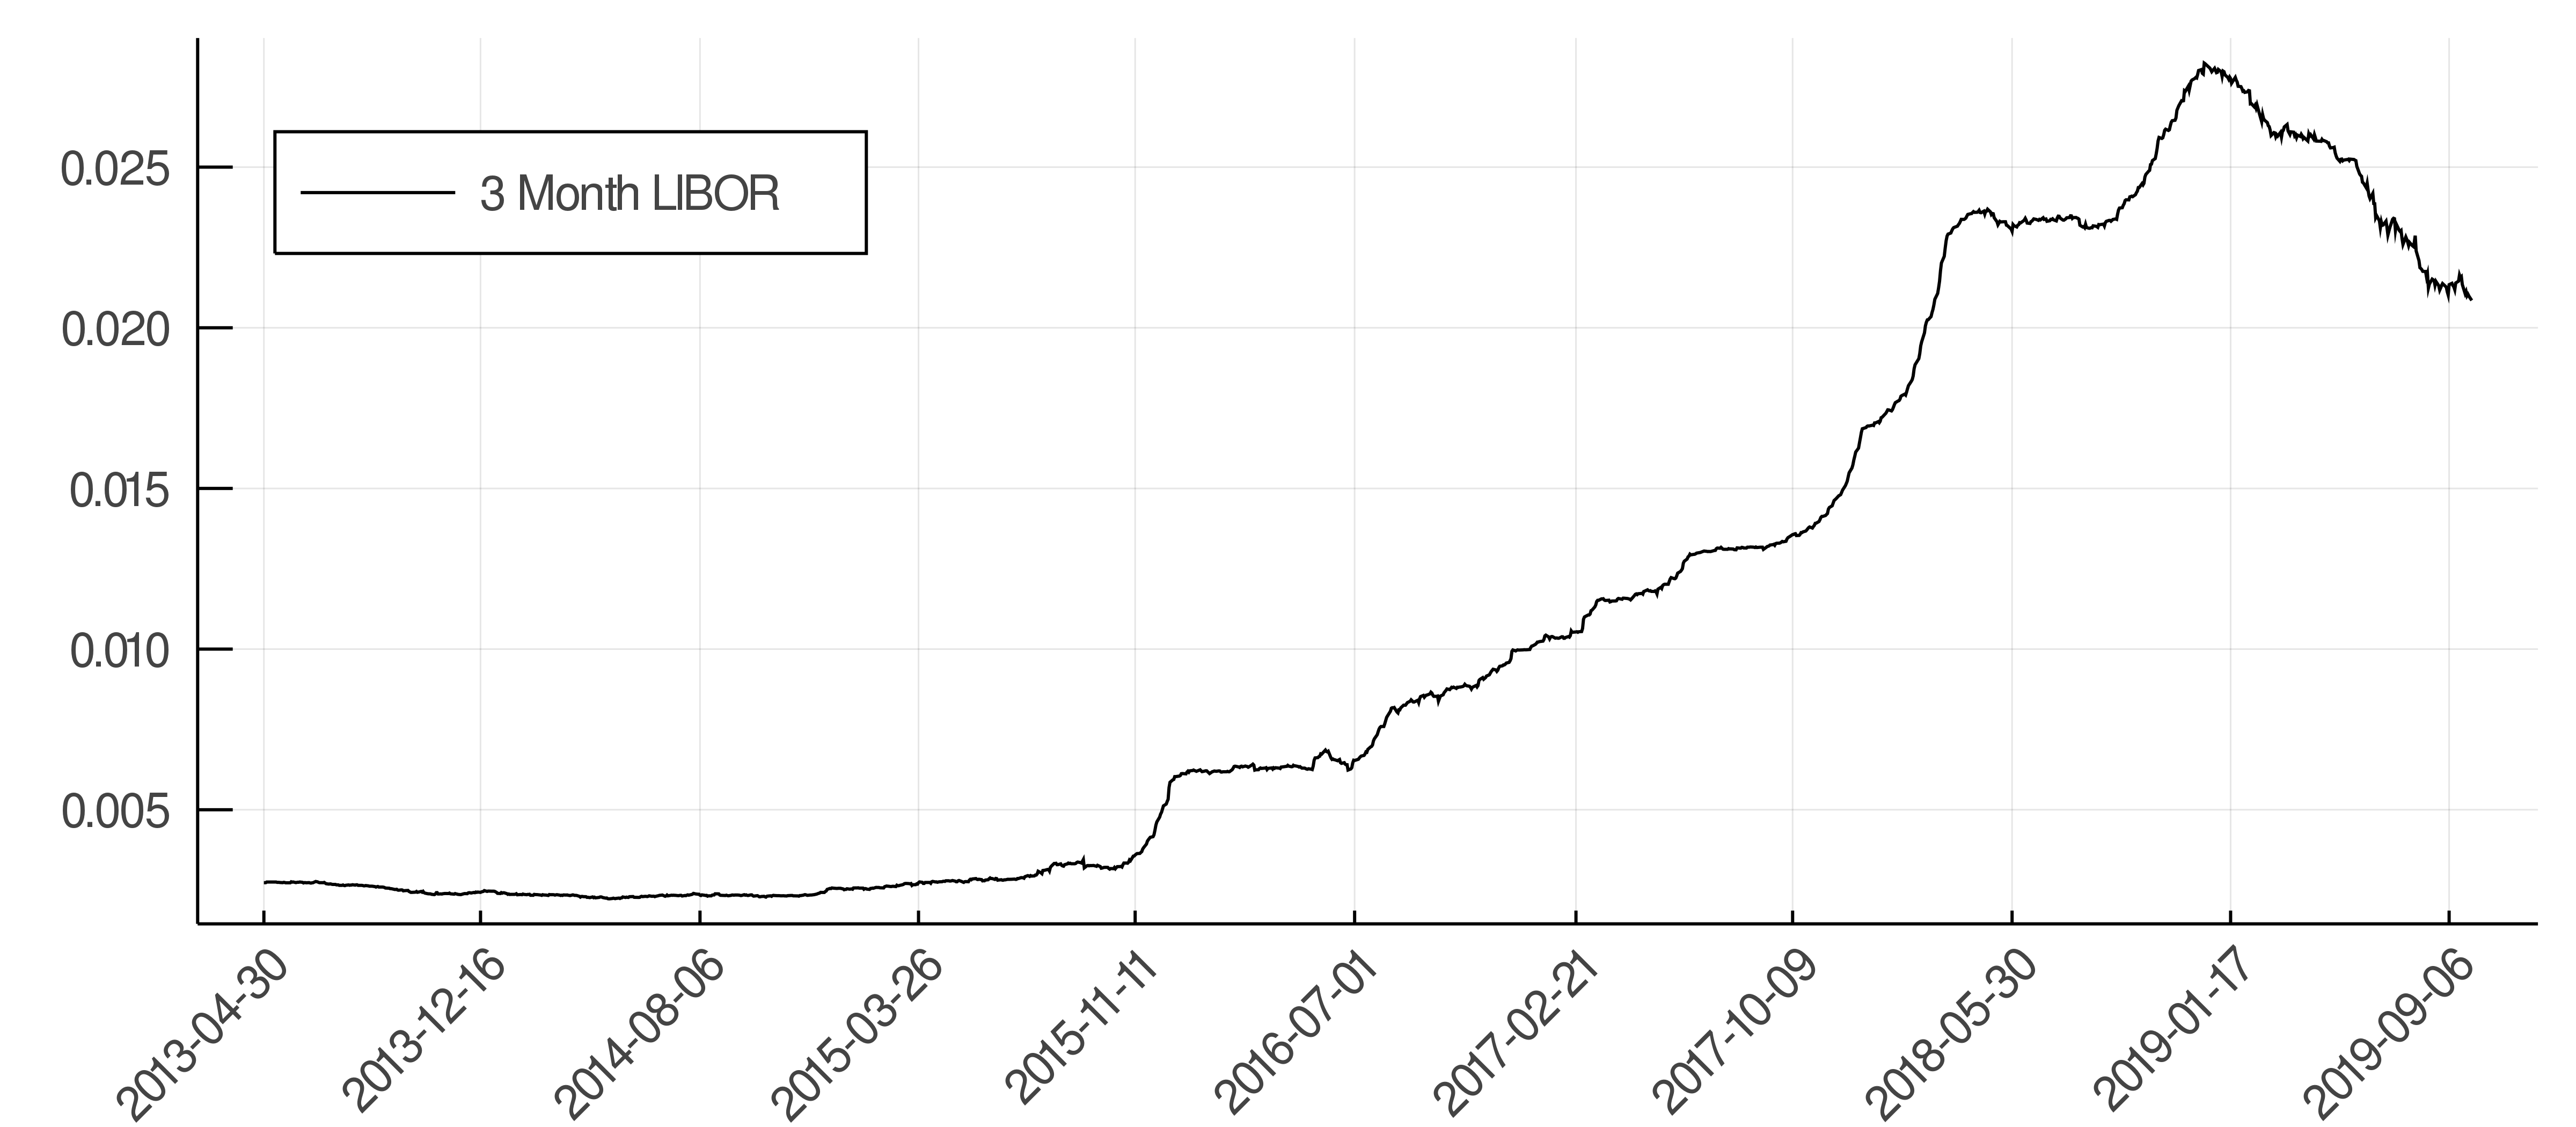
\includegraphics[width=.9\linewidth]{3_month_LIBOR.png}
\caption{Daily 3-month LIBOR rates from the FRED database \url{https://fred.stlouisfed.org/}.}
\label{fig:3}
\end{figure}

\section{Data Summary and Feature Engineering}
\subsection*{Data Summary}
We only considered dates at which we had data for each of these inputs which was delimeted by the number of trading days per year (252). Throughout our data collection process the most common issue we faced was missing data points. This was apparent after we initially plotted the US inflation rates over time and there was sudden drops from 1.5\% to 0.0\% in one day, which happened in 11 data points out of 1617 (0.6\%) in this specific data series. We resolved this issue by linearly interpolating the missing data point, calculating the median of the day prior and the day after the missing data point. We also ran into the same issue after we initially plotted spot gold price over time. In this data series we had 24 data points out of 1617 missing (1.5\%), which we resolved through linear interpolation utilizing the same method as was used for missing inflation rate data. We did not run into data corruption issues.
\subsection*{Feature Engineering}
We have 1617 daily data points for each of our explanatory variables and for bitcoin pricing. Currently we are considering 5 explanatory variables. After transformations we will have a total of 18 explanatory variables to consider.
We have added features for the logarithmic returns of assets for bitcoin, Nvidia, GSPC and gold. We chose to calculate daily returns using a logarithmic basis, calculated by the $ln((today's price / yesterday's price))$. We chose this metric as it presents returns in an additive way, that is if today's return is .01 and yesterday's return was .01, we in total have a .02 return. This is not this case in calculating returns using $(today's price - yesterday's price) / yesterday's price$. This will be important for our calculations if we consider returns daily over a long period of time. Another feature transformation we added was an auto-regressive term for each of our variables that is lagged 30 days. 

\section{Exploratory Data Analysis}
After feature engineering, we first show the fluctuation of the data by visualizing the distribution of the daily returns (Figure 5) generated in the previous section. We notice that the bitcoin price has the largest daily fluctuations compared to the feature variables. This indicates the bitcoin price forming is complicated and we do not have enough features to capture the bitcoin pricing at this point.

We also do a correlation analysis between the features, shown in Figure 4. It is shown that the bitcoin price has relatively strong correlation with the GSPC price, NVDA price, and the 3-month LIBOR. These findings illuminate the feasibility of our study. 

\begin{figure*}[tbhp]
\centering
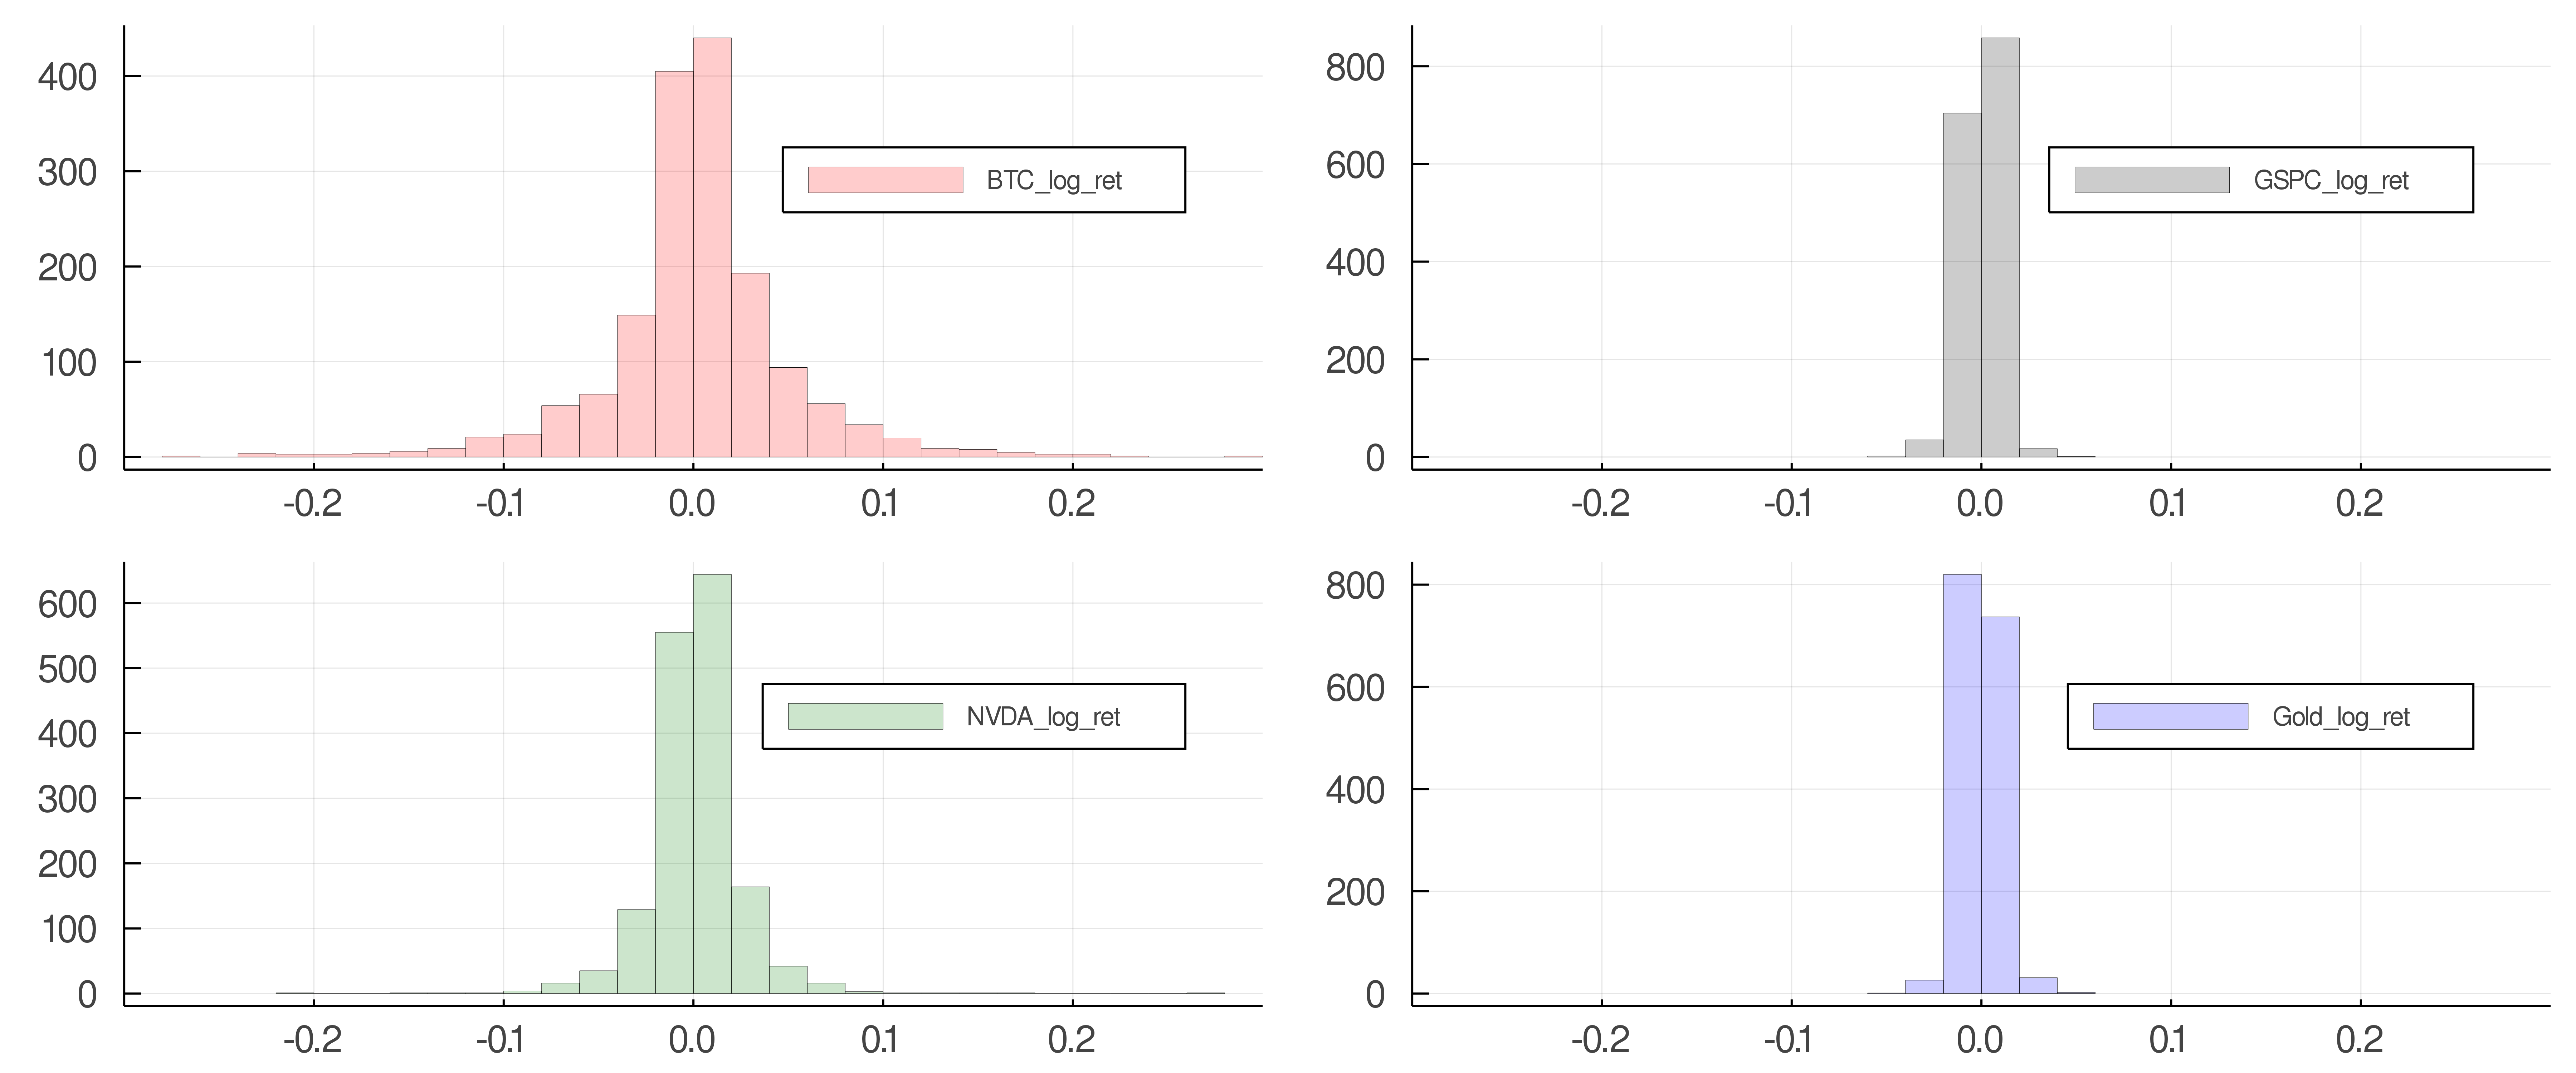
\includegraphics[width=0.9\linewidth]{return_hists.png}
\caption{Histograms showing the distributions of the return rate of bitcoin price, GSPC price, NVDA price and gold price.}
\label{fig:4}
\end{figure*}

\begin{figure}[tbhp]
\centering
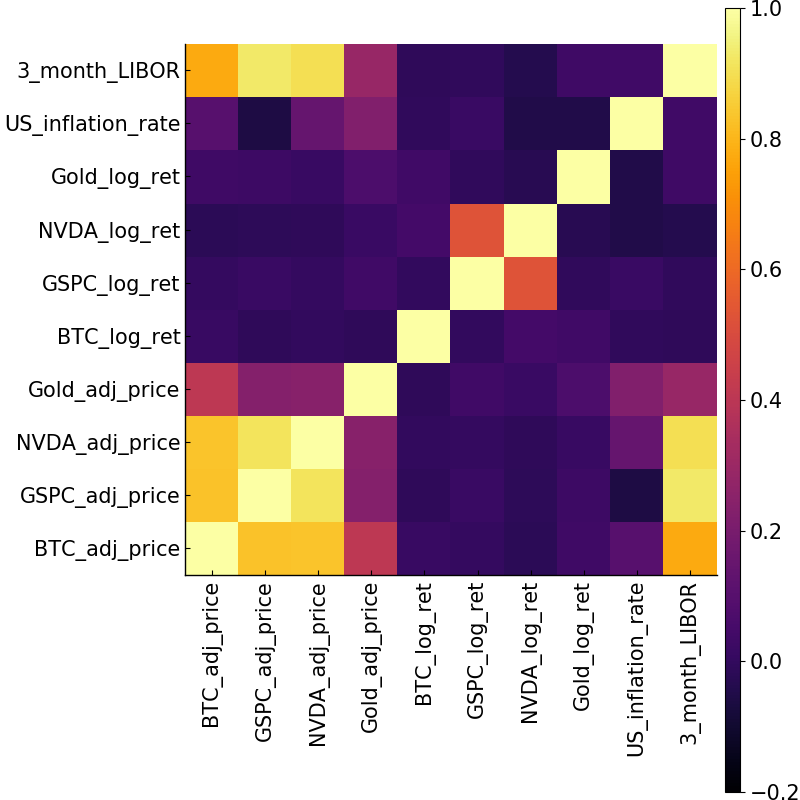
\includegraphics[width=0.8\linewidth]{heatmap.png}
\caption{Correlations between the features and the bitcoin price.}
\label{fig:5}
\end{figure}

\section{Preliminary Learning Practice}
The data we have is a time series. Thus, the first 80\% of the data are put into $\mathcal{D}_{train}$ while the most recent 20\% of the data are put into $\mathcal{D}_{test}$. The simple linear regression results without transformations are shown in Figure 6. Finally we considered a regression using all of our transformations, including the logarithmic returns and auto-regressive variables using a 30 day lag (Figure 7).

\begin{figure}[tbhp]
\centering
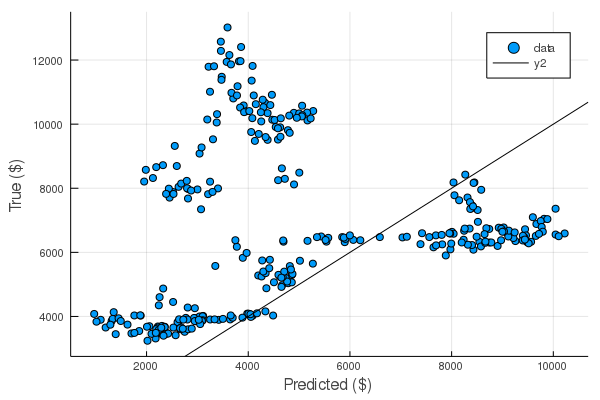
\includegraphics[width=1.0\linewidth]{Regression_wo_all_explanatory.png}
\caption{Regression without transformations.}
\label{fig:9}
\end{figure}

\begin{figure}[tbhp]
\centering
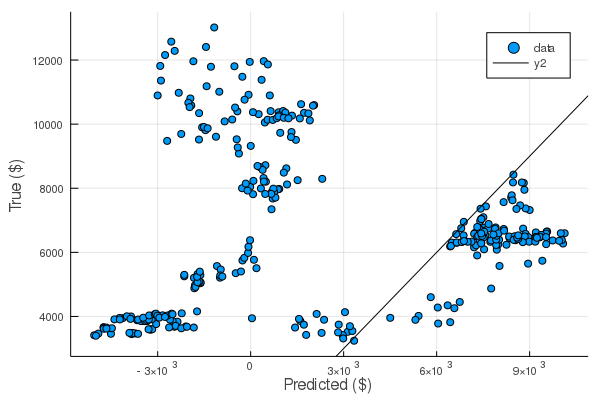
\includegraphics[width=1.0\linewidth]{Regression_w_all_explanatory.png}
\caption{Regression including logarithmic returns and auto-regressive terms.}
\label{fig:10}
\end{figure}

Clearly, such model does not generalize with our data set. A first observation could be there is over-fitting happening. Also, with the transformed features, the model even predicts negative values of bitcoin prices. We check the weights calculated from linear regression, and we found some of the values in the weights are very negative. This means the problem we have could possibly be an under-determined least square problem. This can be revealed by revisiting the data we have in Figure 1 and 2: in history, there can be more than one date that has the same bitcoin price, and the values of other variables during these days cannot be the same. 

\section{Discussion and Future Work}
\subsection*{Discussion}
Given that we have 1617 total data points and 5 explanatory variables, we believe initially we face an issue of under-fitting with our model. We plan to bridge this gap with the addition of new features, more specifically touched on in the section below. We plan to combat over-fitting by removing variables which have a low correlation with bitcoin pricing and therefore are unlikely to help predict future pricing at the cost of adding another level of complexity to our model. We will monitor the change in training vs test set error between models to track when our models appear to be over-fitting versus when they are generalizing.

\subsection*{Future Work}
From the preliminary learning practice, we notice that the problem could be under-determined, so we will try ridge regression instead of the simple least squares. To do this, we will take the advantage of the open source code that solves regularized empirical risk minimization (ERM) problems.

We also consider making the return rate of bitcoin price as a quantity to predict. The return rate basically reflects the price variation during a short term, and that is of great interest because one can utilize it to predict his/her real-time gain when holding the bitcoin. Even the exact quantity of the return can be trivial: we can only focus on its sign, say, if the bitcoin price increase or decrease the next day. 

Thus, the problem could be a classification problem, and we can use logistic loss function to predict the sign of the return rate in a probabilistic manner. As long as the model is believed to have a more than 50\% accuracy, the model is nontrivial, in the long run. Also, as a classification problem, it is easier for us to analyze the generalization properties of the model quantitatively using Hoeffding Bound/VC dimensions.

% Bibliography

\bibliography{bibliography}

\end{document}